\documentclass[9pt]{beamer}
\beamertemplatenavigationsymbolsempty

\usepackage{subfig}
%\usetheme{Berlin}

\definecolor{TriangleColor}{RGB}{255,170,128} % Soft Coral
\definecolor{LineColor}{RGB}{0,128,128} % Darker Blue
\definecolor{VertexColor}{RGB}{255,255,128} % Light Yellow


\usepackage{etex, tikz, array, graphics, xspace, relsize, multirow}
\usepackage{ulem}
\usepackage{faktor} 

\usetikzlibrary{arrows}
\usetikzlibrary{tikzmark}
\input binhex

\makeatletter
\PassOptionsToPackage{sortcites,isbn=false}{biblatex}


% Set frame title color
\setbeamercolor{frametitle}{fg=LineColor}

% Set section title color  
\setbeamercolor{title}{fg=LineColor}



\renewenvironment{theorem}[1][]
{\textcolor{LineColor}{\textbf{Theorem #1}} }
{}

\renewenvironment{definition}[1][]
{\textcolor{LineColor}{\textbf{Definition #1}} }
{}

\renewenvironment{problem}[1][]
{\textcolor{LineColor}{\textbf{Problem #1}} }
{}

\renewenvironment{lemma}[1][]
{\textcolor{LineColor}{\textbf{Lemma #1 }} }
{}

% Set subtitle color
\setbeamercolor{subtitle}{fg=LineColor}

% Set author color
%\setbeamercolor{author}{fg=purple}

% Set institute color
%\setbeamercolor{institute}{fg=orange}

% Set date color
%\setbeamercolor{date}{fg=brown}

\usepackage{enumitem}
\setlist[itemize]{label=\textcolor{LineColor}{\textbullet}}
%\PassOptionsToPackage{inline}{enumitem}
\PassOptionsToPackage{hyperfootnotes=false}{hyperref}
\PassOptionsToPackage{capitalise}{cleveref}
\usepackage{bbding}
\usepackage{pdflscape}
\usepackage{rotating}\setlength{\rotFPtop}{0pt plus 1fil}
\usepackage{layout}
\overfullrule=1ex


\usepackage[textsize=tiny]{todonotes}
\setlength{\marginparwidth}{1.75cm}
\setlength{\marginparsep}{1mm}


% Data tables
\usepackage{siunitx}
\sisetup{reset-math-version = false}
\sisetup{table-auto-round}
\usepackage{xstring}

\usepackage[legacy]{csvsimple}

\sisetup{reset-math-version = false}
\sisetup{table-auto-round}

% For code inclusion
\usepackage{listings}
\lstset{ breaklines=true}
\lstset{escapeinside={<@}{@>}}
\usepackage{algorithm,algorithmic}

\renewcommand{\algorithmicrequire}{\textbf{Input:}}
\renewcommand{\algorithmicensure}{\textbf{Output:}}



\usepackage{svg}
\usepackage{nicematrix}

\usepackage[legacy]{csvsimple}

% For drawing
%% Tikz drawing
\usepackage{tikz} \usetikzlibrary{arrows} \usetikzlibrary{arrows.meta}
\usepackage{pgfplots} \usepackage{tikz-3dplot} \usepackage{tcolorbox}
\usetikzlibrary{matrix,fit,positioning,shapes.geometric,patterns,backgrounds}
\usetikzlibrary{decorations.pathreplacing}
\usetikzlibrary{decorations.markings} \usetikzlibrary{arrows,calc}
\tikzstyle{bigbox} = [draw=blue!50, thick, rounded corners, rectangle]
\tikzset{ >=stealth' } \tikzset{->-/.style={decoration={ markings,
      mark=at position #1 with {\arrow{>}}},postaction={decorate}}}

%% Software names
\newcommand\topcom{\texttt{TOPCOM}\xspace}
\newcommand\mptopcom{\texttt{MPTOPCOM}\xspace}
\newcommand\mptopcomone{\texttt{MPTOPCOM-1}\xspace}
\newcommand\mts{\texttt{mts}\xspace}
\newcommand\mplrs{\texttt{mplrs}\xspace}
\newcommand\soplex{\texttt{soplex}\xspace}
\newcommand\openmpi{\texttt{OpenMPI}\xspace}
\newcommand\mpi{\texttt{MPI}\xspace}
\newcommand\gfan{\texttt{Gfan}\xspace}
\newcommand\cddlib{\texttt{cddlib}\xspace}
\newcommand\polydb{\texttt{PolyDB}\xspace}
\newcommand\Julia{\texttt{Julia}\xspace}

\usepackage{xcolor}
\definecolor{green}{rgb}{0.1,0.59,0.1}
\definecolor{yellow}{rgb}{0.8,0.67,0}
\definecolor{red}{rgb}{0.89,0.1,0.1}
\definecolor{blue}{rgb}{0.1,0.1,0.89}

\usenavigationsymbolstemplate{}

\usepackage{booktabs}
% For software citations
\newcommand{\singular}{\texttt{Sin\-gu\-lar}\xspace}
\newcommand\CPP{C\nolinebreak\hspace{-.05em}\raisebox{.4ex}{\relsize{-3}{\textbf{+}}}\nolinebreak\hspace{-.10em}\raisebox{.4ex}{\relsize{-3}{\textbf{+}}}\xspace}

\usepackage{amsmath}
% Newcommands specifically for this article
\newcommand{\eval}{v}               % evaluation function giving switch table
\newcommand{\graph}{\Gamma}         % reverse search graph
\newcommand{\group}{G}              % group acting on point config
\newcommand{\groupElem}{g}          % element of group
\newcommand{\jbound}{\psi}          % bound on the number of elements of set J
\newcommand{\switchTableSize}{\mu}  % index of last non-trivial row in switch table
\newcommand{\mrdi}{\texttt{mrdi}\xspace}
\newcommand{\OSCAR}{\texttt{OSCAR}\xspace}


\DeclareMathOperator{\CaDiv}{CaDiv}
\DeclareMathOperator{\conv}{conv}
\DeclareMathOperator{\below}{defect}
\DeclareMathOperator{\vertex}{vertex}
\DeclareMathOperator{\Cox}{Cox}
\DeclareMathOperator{\cl}{cl}
\DeclareMathOperator{\cone}{cone}
\DeclareMathOperator{\Ext}{Ext}
\DeclareMathOperator{\Tor}{Tor}
\DeclareMathOperator{\lcm}{lcm}
\DeclareMathOperator{\Quot}{Quot}
\DeclareMathOperator{\Spec}{Spec}
\DeclareMathOperator{\Sets}{Sets}
\DeclareMathOperator{\relint}{relint}
\DeclareMathOperator{\smallestFace}{smallestFace}
\DeclareMathOperator{\Pic}{Pic}
\DeclareMathOperator{\Hom}{Hom}
\DeclareMathOperator{\vol}{vol}
\DeclareMathOperator{\TV}{TV}
\DeclareMathOperator{\tail}{tail}
\DeclareMathOperator{\rep}{rep}
\DeclareMathOperator{\vspan}{span}
\DeclareMathOperator{\canonical}{can}
\DeclareMathOperator{\gkz}{gkz}

\newcommand{\pmsmall}{
\includegraphics[scale=0.03]{pmlogo.png}}
\newcommand{\pmlogo}{
\includegraphics[scale=0.09]{pmlogo.png}}
\newcommand{\pmbluesmall}{\includegraphics[scale=0.03]{pmbluelogo.png}}
\newcommand{\Disjoint}{\mathop{\coprod}}
\newcommand{\Discriminant}{\mathcal{D}}

\author[Antony Della Vecchia]{\textbf{Antony Della Vecchia}, Michael Joswig and Benjamin Lorenz} 
\title{The \mrdi File Format}


\institute[]{
  TU Berlin
}
\date{
  2026-07-01
}
\logo{
  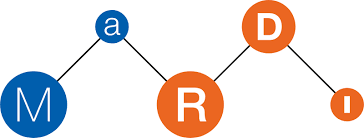
\includegraphics[width=2cm]{images/mardi-logo.png}
}


\newcommand{\surj}{\twoheadrightarrow}
\newcommand{\oursetting}[1]{\textcolor{blue}{#1}}

% Itemize that spreads its items to fill the frame vertically
\newenvironment{fillitemize}
  {\vspace{\fill}\begin{itemize}\setlength{\itemsep}{\fill}}
  {\end{itemize}\vspace{\fill}}

\begin{document}
\maketitle
%%%%%%%%%%%%%%%%%%%%%%%%%%%%%%%%%%%%%%%%%%%%%%%%%%%%%%%%%%%%%%%%%%%%%%%%%%%%%%% 
%%%%%%%%%%%%%%%%%%%%%%%%%%%%%%%%%%%%%%%%%%%%%%%%%%%%%%%%%%%%%%%%%%%%%%%%%%%%%%% 
%%%%%%%%%%%%%%%%%%%%%%%%%%%%%%%%%%%%%%%%%%%%%%%%%%%%%%%%%%%%%%%%%%%%%%%%%%%%%%%

\begin{frame}[fragile]{MaRDI}
  \textbf{Mathematical Research Data Initiative} --- part of Germany's NFDI,
  building research-data infrastructure for mathematics. \pause
  \vfill
  The \textbf{Computer Algebra} task area, led by PIs
  \textbf{Michael Joswig} (TU Berlin) and \textbf{Claus Fieker}
  (RPTU Kaiserslautern), runs four projects: \pause
  \begin{itemize}
  \item \textbf{File format} --- Antony Della Vecchia (TU Berlin) 
  \item \textbf{Guidelines for reproducible workflows} --- Lars Kastner (TU Berlin) 
  \item \textbf{Technical peer review} --- Jeroen Hanselmann (RPTU Kaiserslautern) 
  \item \textbf{Containerization} --- Aaruni Kaushik (RPTU Kaiserslautern)
  \end{itemize}
\end{frame}

%%%%%%%%%%%%%%%%%%%%%%%%%%%%%%%%%%%%%%%%%%%%%%%%%%%%%%%%%%%%%%%%%%%%%%%%%%%%%%%

\begin{frame}[fragile, t]{Infrastructure}
  \begin{fillitemize}
  \item In mathematics, a theorem from another field is never off-limits:
    if it applies to your work, you use it. \pause
  \item Software should be the same --- a result computed in one system should
    not be locked out of another. \pause
  \item To support these ideas we need infrastructure.

  \item Software infrastructure is important for research --- but is often overlooked and underfunded. \pause
  \item The tools mathematicians compute with deserve the same care as the
    mathematics itself. \pause

  \end{fillitemize}
\end{frame}

%%%%%%%%%%%%%%%%%%%%%%%%%%%%%%%%%%%%%%%%%%%%%%%%%%%%%%%%%%%%%%%%%%%%%%%%%%%%%%%
%%%%%%%%%%%%%%%%%%%%%%%%%%%%% SECTION 1: HISTORY %%%%%%%%%%%%%%%%%%%%%%%%%%%%%%
%%%%%%%%%%%%%%%%%%%%%%%%%%%%%%%%%%%%%%%%%%%%%%%%%%%%%%%%%%%%%%%%%%%%%%%%%%%%%%%

\section{A History of File Formats}

\begin{frame}[fragile, t]{Why Files?}
  \begin{fillitemize}
  \item People often have a preferred software system. \pause
  \item Computations can be expensive. \pause
  \item Verification of results is at most as computationally expensive. \pause
  \item Software changes often.
  \item Example: Surfaces in $\mathbb{P}^4$
  \end{fillitemize}
\end{frame}

%%%%%%%%%%%%%%%%%%%%%%%%%%%%%%%%%%%%%%%%%%%%%%%%%%%%%%%%%%%%%%%%%%%%%%%%%%%%%%%


\begin{frame}[fragile]{A History of File Formats}

  \begin{tabular}{cl}
    \begin{tabular}{c}
      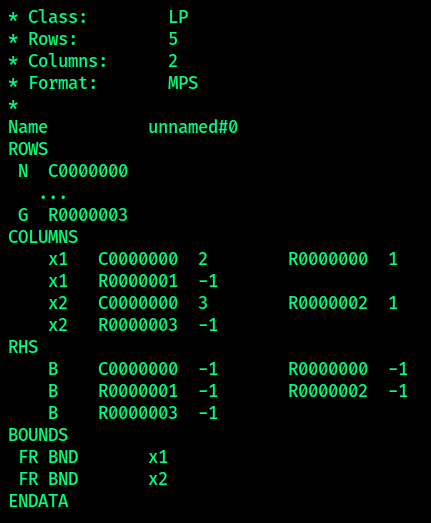
\includegraphics[width=.45\textwidth]{images/mps_file}
    \end{tabular}
    & \begin{tabular}{l}
      \parbox{0.38\linewidth}{%
      \begin{itemize}
      \item The LP and MPS file formats. IBM [1970s] (industry standards)
      \item \texttt{Mathematica} Notebooks. Wolfram [1988]
      \item \textbf{\texttt{OpenMath}} (tree structure). Mike Dewar [2000]
      \item \texttt{IPython 0.12} interactive browser notebooks (Jupyter) [2011]
      \item \texttt{polymake} file format. Gawrilow, Hampe, Joswig [2016]
      \end{itemize}
      }
    \end{tabular}  \\
  \end{tabular}
\end{frame}

%%%%%%%%%%%%%%%%%%%%%%%%%%%%%%%%%%%%%%%%%%%%%%%%%%%%%%%%%%%%%%%%%%%%%%%%%%%%%%%

\begin{frame}[fragile]{Storing Computer Algebra Data}
  \begin{itemize}
  \item It's common to have multiple perspectives on an object in mathematics.
  \item While storing mathematical data a choice of perspective must be made.
  \item Such a choice might not be describable in an email.
  \end{itemize}

  Say we want to store:
  \begin{align*}
    p = 2y^3z^4 + (\mathbf{a} + 3)z^2 + 5\mathbf{a}y + 1
  \end{align*} \pause

  \begin{itemize}
  \item Some technicalities with the coefficients.
  \item Is $y$ considered a coefficient of $z$?
  \item What is $\mathbf{a}$? \pause
  \item How can we guarantee the objects behave as expected on load?
  \end{itemize}
\end{frame}

%%%%%%%%%%%%%%%%%%%%%%%%%%%%%%%%%%%%%%%%%%%%%%%%%%%%%%%%%%%%%%%%%%%%%%%%%%%%%%%
%%%%%%%%%%%%%%%%%% SECTION 2: OPENMATH / FATEMAN (TODO) %%%%%%%%%%%%%%%%%%%%%%%
%%%%%%%%%%%%%%%%%%%%%%%%%%%%%%%%%%%%%%%%%%%%%%%%%%%%%%%%%%%%%%%%%%%%%%%%%%%%%%%

\section{OpenMath (2000): A Top-Down Approach}

\begin{frame}[fragile]{\texttt{OpenMath}: A Top-Down Approach}
  \begin{itemize}
  \item Goal: a software-independent standard for the \emph{meaning} of
    mathematical objects, not just their syntax. \pause
  \item An \texttt{OpenMath} object is a tree of symbols, each defined in a
    \textbf{Content Dictionary}. \pause
  \item Top-down: agree on the semantics of \emph{all} of mathematics first,
    then every system speaks the same language. \pause
  \end{itemize}
  \textbf{Fateman's critique:}
  \begin{itemize}
  \item Formalising the semantics of all mathematics is open-ended, and meaning
    is context-dependent --- there is no single agreed semantics. \pause
  \item Using the semantics means reimplementing every Content Dictionary ---
    in effect, building a whole separate computer algebra system to read a file.
  \end{itemize}
  \vfill
  {\footnotesize R. Fateman, \emph{A Critique of \texttt{OpenMath} and Thoughts
    on Encoding Mathematics}.}
\end{frame}

%%%%%%%%%%%%%%%%%%%%%%%%%%%%%%%%%%%%%%%%%%%%%%%%%%%%%%%%%%%%%%%%%%%%%%%%%%%%%%%
%%%%%%%%%%%%%%%%%%%%%%% SECTION 3: THE mrdi FORMAT (TODO) %%%%%%%%%%%%%%%%%%%%%
%%%%%%%%%%%%%%%%%%%%%%%%%%%%%%%%%%%%%%%%%%%%%%%%%%%%%%%%%%%%%%%%%%%%%%%%%%%%%%%

\begin{frame}[fragile]{A Bottom Up Approach}
  \textbf{What is a bottom-up approach?} \pause
  \begin{itemize}
  \item No attempt to formalise the language of mathematics up front. \pause
  \item Semantics come from the software that produces the data, not from a
    global specification. \pause
  \item The format grows from real data and real software, rather than the
    other way around. \pause
  \end{itemize}
  \vfill
  \textbf{What features do we need to support it?} \pause
  \begin{itemize}
  \item \textbf{Namespaces} to pin semantics to a specific software and version. \pause
  \item \textbf{Open source implementations} of saving and loading. \pause
  \item \textbf{Versioning and upgrades}: older files are upgraded on load. \pause
  \end{itemize}
\end{frame}


%%%%%%%%%%%%%%%%%%%%%%%%%%%%%%%%%%%%%%%%%%%%%%%%%%%%%%%%%%%%%%%%%%%%%%%%%%%%%%%

\section{The \texttt{mrdi} File Format}

\begin{frame}[fragile]{The \mrdi File Format}
  \begin{tcolorbox}[]
    \begin{itemize}
    \item Based on JSON (tree structure). \pause
    \item Generalizes ideas from the \texttt{polymake} format to algebraic data. \pause
    \item Namespaces pin semantics to a specific software. \pause
    \item References to shared parent types, stored with UUIDs. \pause
    \item First version developed using \OSCAR.
    \end{itemize}
  \end{tcolorbox}
\end{frame}

%%%%%%%%%%%%%%%%%%%%%%%%%%%%%%%%%%%%%%%%%%%%%%%%%%%%%%%%%%%%%%%%%%%%%%%%%%%%%%%

\begin{frame}[fragile]{Tree Structure}
  \vspace*{-0.5cm}
  \begin{tabular}{cl}
    \begin{tabular}{c}
      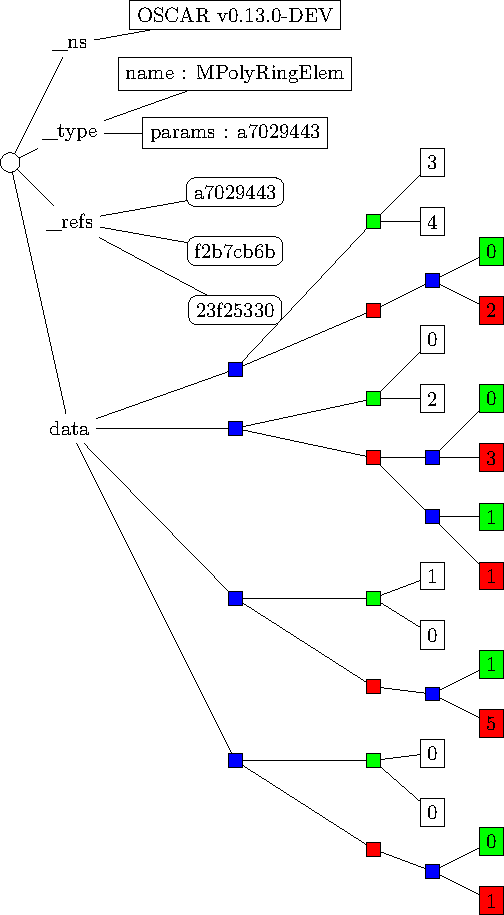
\includegraphics[width=0.43\textwidth, height=0.8\textheight]{images/tree-coloured}
    \end{tabular}
    & \begin{tabular}{l}
      \parbox{0.25\linewidth}{%
      \begin{align*}
        \\ \\ \\
        & 2y^3z^4 \\
        \\ \\
        &  (a + 3)z^2 \\
        \\ \\
        & 5ay \\
        \\ \\
        & 1
      \end{align*}
      }
    \end{tabular}  \\
  \end{tabular}
\end{frame}

%%%%%%%%%%%%%%%%%%%%%%%%%%%%%%%%%%%%%%%%%%%%%%%%%%%%%%%%%%%%%%%%%%%%%%%%%%%%%%%

\begin{frame}[fragile]{Example File Serialized with \OSCAR}
  \begin{center}
    
\includegraphics[height=0.9\textheight]{images/polynomial-example}
  \end{center}
\end{frame}

%%%%%%%%%%%%%%%%%%%%%%%%%%%%%%%%%%%%%%%%%%%%%%%%%%%%%%%%%%%%%%%%%%%%%%%%%%%%%%%

\begin{frame}[fragile]{Shared Parents Across Sessions}
  Save two polynomials --- the shared ring is stored once, referenced by UUID:
  \begin{lstlisting}[basicstyle=\ttfamily\footnotesize]
julia> R, (y, z) = polynomial_ring(QQ, [:y, :z]);

julia> save("p.mrdi", 2*y^3*z^4 + 3*z^2 + 5*y + 1)

julia> save("q.mrdi", y + 1)
  \end{lstlisting}
  \pause

  In a \textbf{new session}, load both and multiply --- they share a parent:
  \begin{lstlisting}[basicstyle=\ttfamily\footnotesize]
julia> p = load("p.mrdi");

julia> q = load("q.mrdi");

julia> parent(p) === parent(q)
true

julia> p * q
2*y^4*z^5 + 2*y^3*z^4 + 3*y*z^3 + 5*y^2*z + 3*z^2 + y*z + 5*y + 1
  \end{lstlisting}
\end{frame}

%%%%%%%%%%%%%%%%%%%%%%%%%%%%%%%%%%%%%%%%%%%%%%%%%%%%%%%%%%%%%%%%%%%%%%%%%%%%%%%

\begin{frame}[fragile]{Saving and Loading in \OSCAR}
  Save an object to a \mrdi file and load it back:
  \begin{lstlisting}[basicstyle=\ttfamily\footnotesize]
julia> using Oscar

julia> R, (y, z) = polynomial_ring(QQ, [:y, :z]);

julia> save("poly.mrdi", 2*y^3*z^4 + 3*z^2 + 5*y + 1)

julia> load("poly.mrdi")
2*y^3*z^4 + 3*z^2 + 5*y + 1
  \end{lstlisting}
  \pause

  Override the parent on load --- reinterpret the same data in a new ring:
  \begin{lstlisting}[basicstyle=\ttfamily\footnotesize]
julia> S, (u, v) = polynomial_ring(GF(7), [:u, :v]);

julia> load("poly.mrdi"; params=S)
2*u^3*v^4 + 3*v^2 + 5*u + 1
  \end{lstlisting}
\end{frame}


%%%%%%%%%%%%%%%%%%%%%%%%%%%%%%%%%%%%%%%%%%%%%%%%%%%%%%%%%%%%%%%%%%%%%%%%%%%%%%%
%%%%%%%%%%%%%%%%%%%%% SECTION 4: TODAY AND THE FUTURE (TODO) %%%%%%%%%%%%%%%%%%
%%%%%%%%%%%%%%%%%%%%%%%%%%%%%%%%%%%%%%%%%%%%%%%%%%%%%%%%%%%%%%%%%%%%%%%%%%%%%%%

\section{Today and the Future}

\begin{frame}[fragile]{Where We Are Today}
  \begin{itemize}
  \item All core \OSCAR types can be serialized. \pause
  \item Multiple upgrades to the format. \pause
  \item Multiprocess computing backed by the format. \pause
  \item Growing interest from other computer algebra systems: \pause
    \begin{itemize}
    \item \texttt{Macaulay2} 1.26 ships with a \texttt{MRDI} package
      (Doug Torrance): \texttt{saveMRDI} / \texttt{loadMRDI} for $\mathbb{Z}$,
      $\mathbb{Q}$, finite and Galois fields, polynomial rings, ideals,
      matrices. \pause
    \item A \texttt{Magma} implementation by Jeroen Hanselman
      (\texttt{MagmaMaRDI-JSON}): booleans, strings, $\mathbb{Z}$, $\mathbb{Q}$,
      finite fields, polynomial rings, matrices, arrays. \pause
    \item A \texttt{SageMath} implementation (\texttt{SageMathMRDIJSON}, built
      with Claude Code): matrices, polynomial rings and ideals over $\mathbb{Q}$,
      compatible with \OSCAR's format.
    \item Some \texttt{Lean} functionality (Cedric Holler, Doug Torrance)
    \end{itemize}
  \end{itemize}
\end{frame}

%%%%%%%%%%%%%%%%%%%%%%%%%%%%%%%%%%%%%%%%%%%%%%%%%%%%%%%%%%%%%%%%%%%%%%%%%%%%%%%

\begin{frame}[fragile]{Databases and Collections}
  \textbf{OscarDB} --- collections in a MongoDB, queried directly from \OSCAR;
  a RESTful API is coming soon. \pause
  \begin{itemize}
  \item \texttt{SmallTreeModels}
  \item \texttt{SelfProjectingMatroids}
  \item \texttt{LeechPairs} 
  \item \texttt{TransitiveSimplicialComplexes}
  \end{itemize}
  \pause
  \vspace{0.2cm}
  \textbf{Collections shipped with \OSCAR}
  \begin{itemize}
  \item \texttt{ArchimedeanSolids}, \texttt{CatalanSolids},
    \texttt{JohnsonSolids}
  \item \texttt{Surfaces in $\mathbb{P}^4$}, \texttt{TauTaubarGenericEnriquesSurfaces}
  \end{itemize}
\end{frame}

%%%%%%%%%%%%%%%%%%%%%%%%%%%%%%%%%%%%%%%%%%%%%%%%%%%%%%%%%%%%%%%%%%%%%%%%%%%%%%%

\begin{frame}[fragile]{}
  \vfill
  \begin{center}
    \Large Thank you!
  \end{center}
  \vfill
\end{frame}
\end{document}
